\begin{figure}[H]
    \centering
    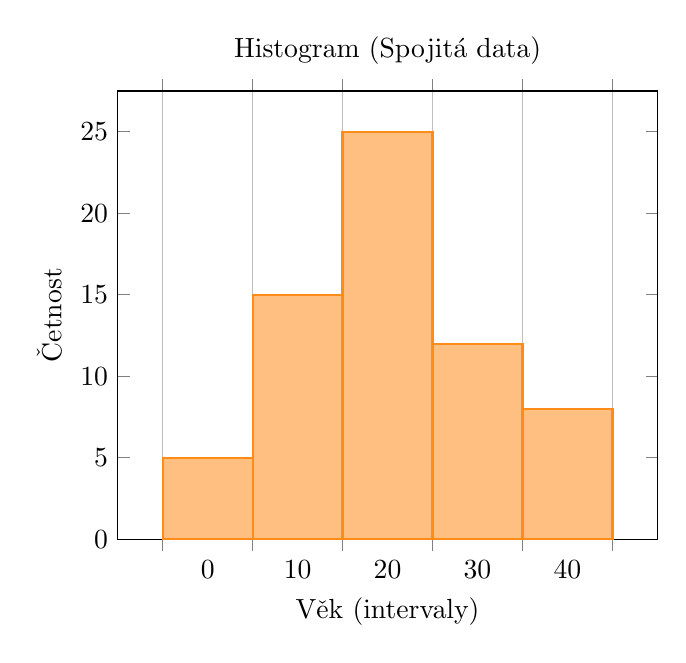
\begin{tikzpicture}
        \begin{axis}[
            ybar interval, % typ grafu: intervalový histogram
            xtick=data,
            ymin=0,
            ylabel={Četnost},
            xlabel={Věk (intervaly)},
            title={Histogram (Spojitá data)}
        ]
            % Souřadnice: (začátek intervalu, výška sloupce). Poslední bod určuje konec osy.
            \addplot[fill=orange!50, draw=orange!90, thick] coordinates {(0, 5) (10, 15) (20, 25) (30, 12) (40, 8) (50, 0)};
        \end{axis}
    \end{tikzpicture}
\end{figure}